% !TEX root = ../../../main.tex

\toggletrue{image}
\toggletrue{imagehover}
\chapterimage{turtles}
\chapterimagetitle{\uppercase{Turtles}}
\chapterimageurl{https://xkcd.com/889/}
\chapterimagehover{\small You're a turtle!}


\chapter{Mein erstes Programm}
\label{ch:mein-erstes-programm}

Folgende Ziele erreichen Sie nach diesem Kapitel:\\

\lernziel[\autoref{part:turtle-programmierung}, Turtle-Programmierung]{\autoref{ch:mein-erstes-programm}, \nameref{ch:mein-erstes-programm}}{
\begin{minipage}{\linewidth}
$\square$ \hspace{0.1cm} Sie erklären, was eine imperative Programmiersprache und ein Programm ist.\\
$\square$ \hspace{0.1cm} Sie erklären, was eine \protect\acs{IDE} ist und warum wir eine \protect\acs{IDE} einsetzen.\\
$\square$ \hspace{0.1cm} Sie erklären, was ein Ordner ist und erstellen einen Ordner auf Ihrem Computer.\\
$\square$ \hspace{0.1cm} Sie erklären, was eine Datei und eine Python-Datei ist.\\
$\square$ \hspace{0.1cm} Sie erstellen eine Python-Datei in einem vorgegebenen Ordner.
\end{minipage}
}

\section{Quadrat zum Ersten}
\label{sec:quadrat-zum-ersten}

\begin{example}

    Unser erstes Python-Programm wird die Turtle dazu anweisen, ein Quadrat zu zeichnen.
    \autoref{lst:quadrat} zeigt die entsprechenden Befehle.


    \begin{figure}[H]
        \centering
        \begin{lstlisting}[language={python3}, caption={Befehle für ein Quadrat (\graybgtexttt{quadrat.py}).}, label={lst:quadrat}]
import turtle

turtle.forward(100)
turtle.left(90)
turtle.forward(100)
turtle.left(90)
turtle.forward(100)
turtle.left(90)
turtle.forward(100)
turtle.left(90)
turtle.done()

\end{lstlisting}
\end{figure}

\begin{hinweis}
    Das Zeichen \lstinline[language={python3}]{ } soll verdeutlichen, dass hier ein Leerzeichen\footnote{Leerschlag} eingegeben werden \textbf{muss}.
    Alle anderen Leerzeichen, die nicht explizit abgedruckt sind, sollten, müssen aber nicht notiert werden.
\end{hinweis}

Wenn Sie das Programm ausführen würden, dann öffnet sich das Fenster aus \autoref{fig:quadrat} und das Quadrat wird von der \say{Turtle} (dem kleinen Dreieck) gezeichnet.

\begin{figure}[htb]
    \centering
    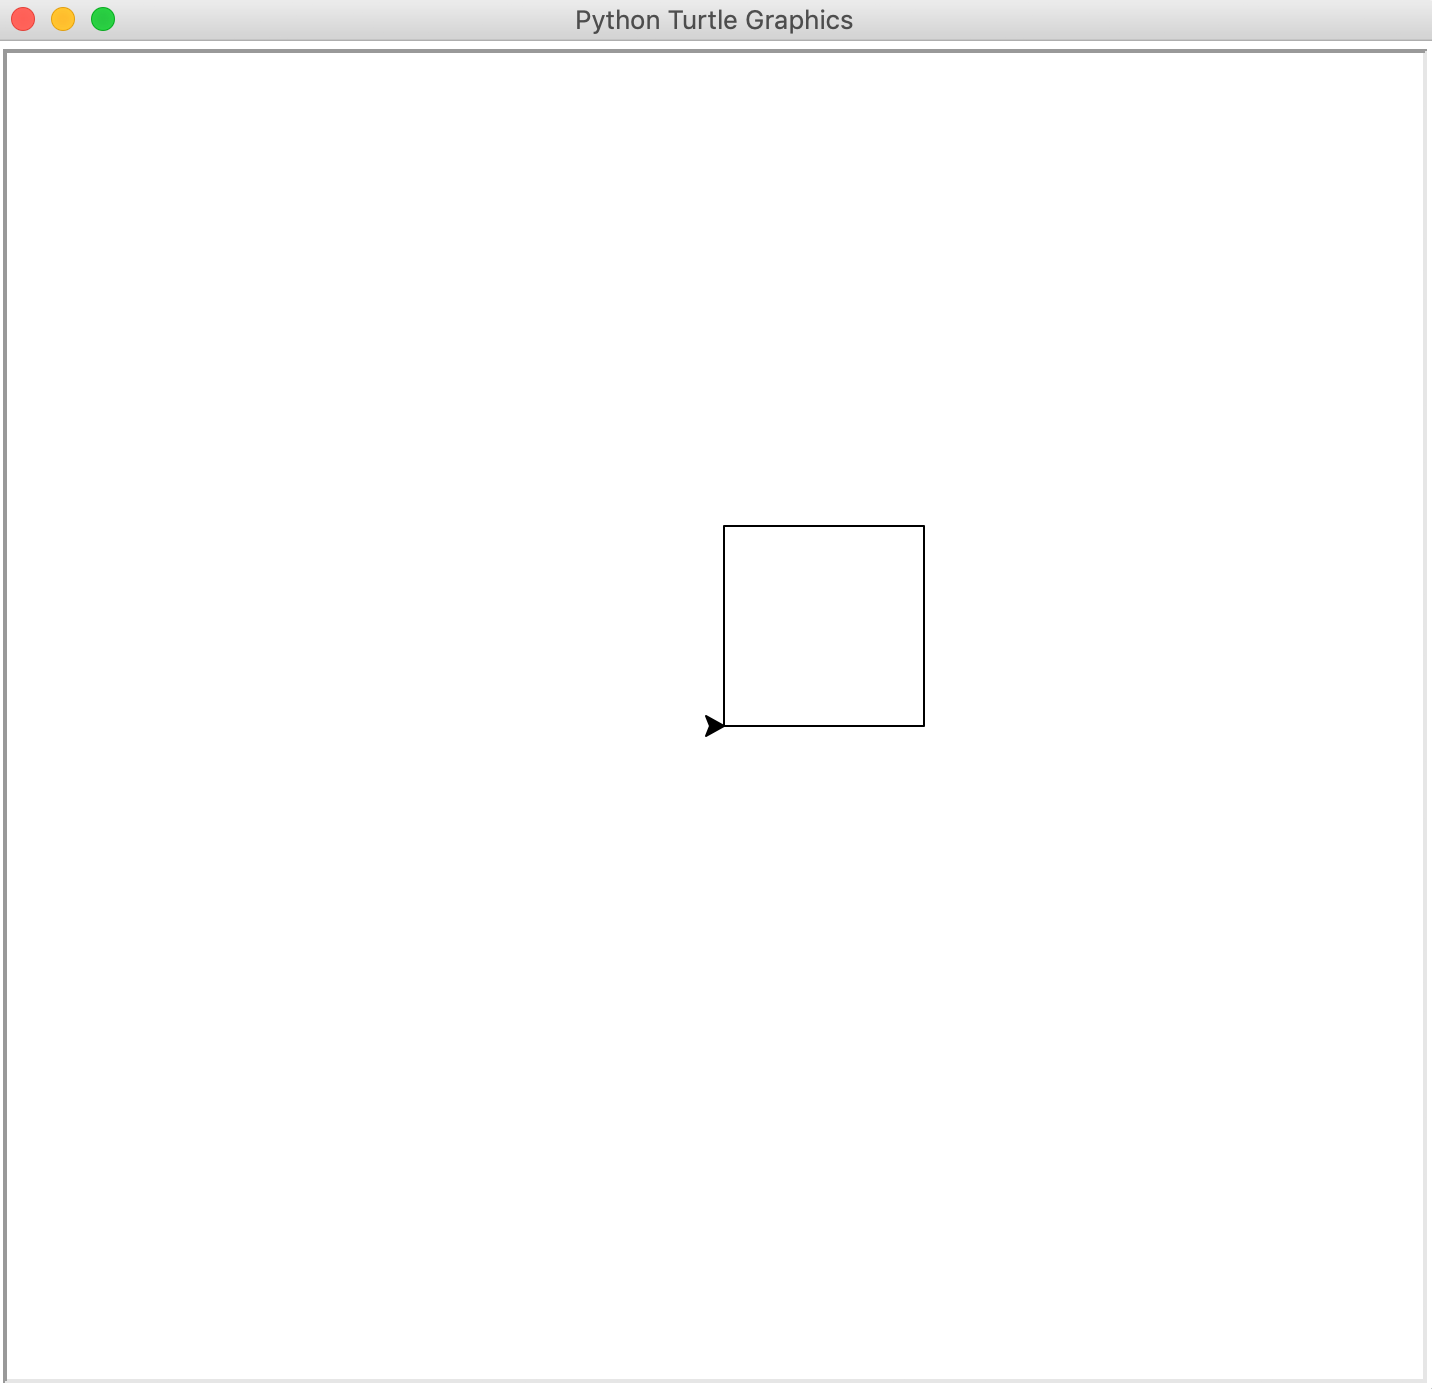
\includegraphics[scale=0.25]{quadrat}
    \caption{Resultat der Ausführung unter macOS.\protect\footnotemark}
    \label{fig:quadrat}
\end{figure}

\end{example}

\footnotetext{Bildquelle: Screenshot des Programms.}

\section{Begriffe}

Wir klären hier zwei typische Begriffe aus dem Programmierumfeld.

\begin{definition}[Listing (dt.: Programmausdruck)]
Bezeichnung für den vollständigen Ausdruck des Source Codes eines Programms auf Papier.
Listings dienen der Dokumentation eines Programms, der Fehlersuche (besserer Überblick über das Programm als auf dem Bildschirm oder bei der Anzeige in einem Debugger) oder zu Lehrzwecken. \cite{def-listing}
\end{definition}

\begin{definition}[Source Code (dt.: Quellcode)]
Bezeichnung für den Programmtext, der ein Programmierer bzw. eine Programmiererin eingegeben hat.
Wird oft einfach mit Code abgekürzt.
\end{definition}

\section{Zusammenfassung}

Typischerweise verwenden wir für das Erstellen eines Textes (z. B. einen Lebenslauf) ein Textverarbeitungsprogramm (z. B. Microsoft Word).
Auch für das Programmieren ist es von Vorteil, wenn wir ein spezielles Programm verwenden.
Ein solches Programm wird \textbf{\ac{IDE}} genannt.
PyCharm ist zum Beispiel eine \ac{IDE} und unterstützt uns beim Programmieren mit Python.
Eine Software zu erstellen, wird häufig auch als Software-Entwicklung (engl. software development) bezeichnet.
In einer \textbf{Datei} (engl. file) kann ein Computeranwender Informationen langfristig auf einem Speichermedium (Festplatte, \ac{USB}-Stick, Cloud etc.) speichern.
Die gespeicherten Informationen können sehr vielseitig sein: Texte, Bilder, Audio, \dots oder auch ein Python-Programm.
Eine Datei, in der ein Python-Programm gespeichert ist, nennen wir \textbf{Python-Datei}.
Eine Datei wird häufig unter Verwendung eines Punktes (\texttt{.}) in zwei Teile gegliedert, den eigentlichen Namen und die sogenannte \textbf{Dateinamen-Erweiterung} (engl. file extension).
Für Word-Dateien gibt es zum Beispiel die Dateinamen-Erweiterung \texttt{.docx}.
Python-Dateien haben die Dateinamen-Erweiterung \texttt{py}. In einem \textbf{Ordner} (engl. directory oder folder) können mehrere Dateien zusammengefasst werden.
Ein Ordner kann wiederum auch einen weiteren Ordner besitzen.